\subsection{Längentreue Kegelprojektion}
\label{sec:langkeg}
Die längentreue Kegelprojektion ist eine globale Projektion. Sie ist weder winkel- noch flächentreu.
Die Verzerrung nimmt zum Kartenrand hin zu. Die Breitenkreise sind in dieser Projektion gleichmäßig verteilt, und die Längenkreise werden als Geraden dargestellt. Die Projektion bildet die Erde auf einen Kegelmantel ab.\\

\begin{figure}[hbtp]
\centering
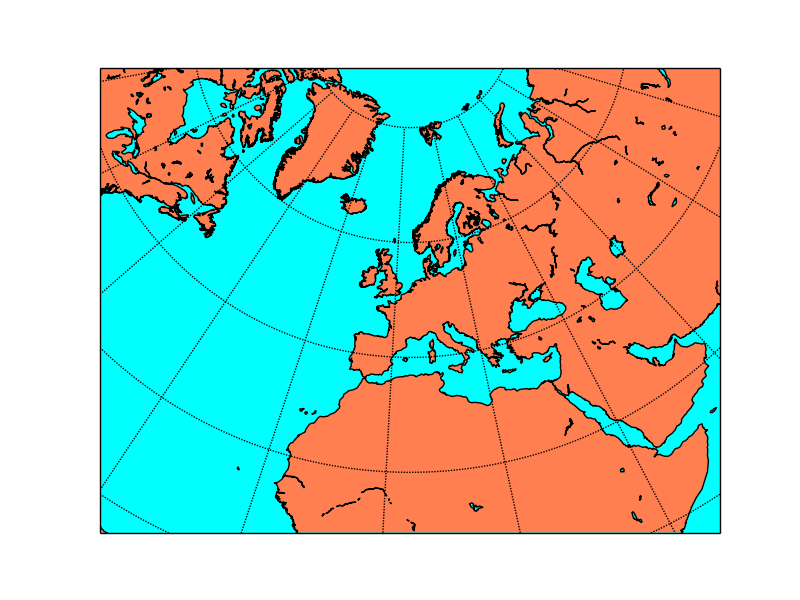
\includegraphics[scale=0.5,origin=c]{/Users/student/seminar/Kartendarstellungen/seminar/eqdc} \caption{Längentreue Kegelprojektion}
\end{figure}
\newpage 